\subsection{Anforderungen der Erklärungen}


\begin{figure}[htb!]
    \centering
    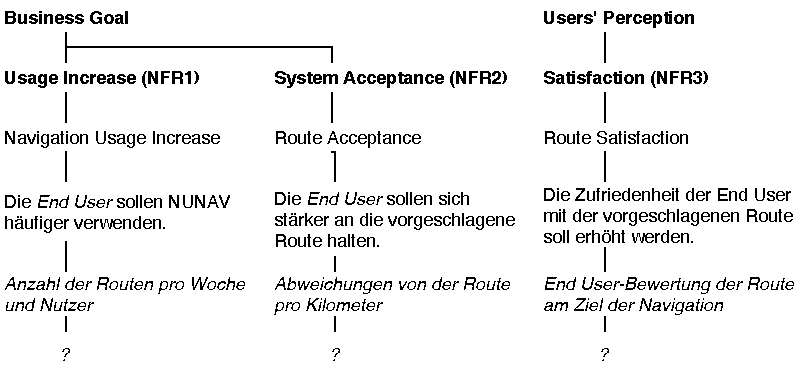
\includegraphics[width=\textwidth]{contents/06_model_evaluation/01_integration/res/quality_model.pdf}
    \caption{Qualitätsmodell für die Integration von Erklärungen in NUNAV Navigation}
    \label{fig:nunav_explanation_quality_model}
\end{figure}

which explanandum X must be explained \cite{kohl_explainability_2019}


\cite{golledge1999wayfinding}

\cite{bovy2012route}

\cite{kohl_explainability_2019} gives a good overview to the requirement analysis for Explainability as an NFR

Formulierung der Anforderungen nach \cite{rajnish2010quality, wiegers1999writing, alexander2002writing} formuliert.

Display context informaiton (Einfach zu integrieren) \cite{wiegand_id_2020}